\documentclass{article}
\usepackage{tikz}
\usetikzlibrary{calc, arrows.meta}
\begin{document}

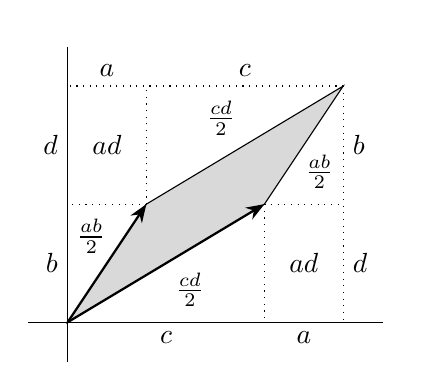
\begin{tikzpicture}
    % Define the scaled coordinates (smaller angle)
    \coordinate (O) at (0,0);
    \coordinate (A) at (1, 1.5);   
    \coordinate (D) at (2.5, 1.5); 
    \coordinate (B) at ($ (A) + (D) $); % (3.5, 3.0)

    % Draw the axes (no arrows)
    \draw (-0.5,0) -- (4,0) node[right] {}; 
    \draw (0,-0.5) -- (0,3.5) node[above] {}; 

    % --- Add specific dotted lines ---
    
    % Original line from A: Vertical line to x-axis
    \draw[dotted] (A) -- (A -| O); 
    
    % Original line from D: Horizontal line to y-axis
    \draw[dotted] (D) -- (D |- O); 
    
    % New line from A: Dotted vertical line upwards
    \draw[dotted] (A) -- (A |- 0, 3); 
    
    % New line from D: Dotted horizontal line to the right
    \draw[dotted] (D) -- (D -| 3.5,0); 
    
    % Both lines from B (vertical to x-axis, horizontal to y-axis)
    \draw[dotted] (B) -- (B -| O); % Vertical
    \draw[dotted] (B) -- (B |- O); % Horizontal
    % --- End of dotted lines ---

    % Draw the parallelogram and fill it with gray
    \fill[gray!30] (O) -- (A) -- (B) -- (D) -- cycle;
    \draw (O) -- (A) -- (B) -- (D) -- cycle;


    % Add arrows for the vectors with -Stealth style
    \draw[-Stealth, thick] (O) -- (A);
    \draw[-Stealth, thick] (O) -- (D);
    
    \node[below] at (1.25,0) {$c$};
    \node[below] at (3,0) {$a$};

    \node[right] at (3.5,0.75) {$d$};
    \node[right] at (3.5,2.25) {$b$};
    
    \node[left] at (0,0.75) {$b$};
    \node[left] at (0,2.25) {$d$};

    \node[above] at (0.5,3) {$a$};
    \node[above] at (2.25,3) {$c$};

    \node at (0.5,2.25) {$ad$};
    \node at (3,0.75) {$ad$};
    \node[above left] at (2.25,2.25) {$\frac{cd}{2}$};
    \node[below right] at (1.25,0.75) {$\frac{cd}{2}$};
    \node[above left,xshift=3pt] at (0.5,0.75) {$\frac{ab}{2}$};
    \node[below right,xshift=-3pt] at (3,2.25) {$\frac{ab}{2}$};
\end{tikzpicture}

\end{document}
